\documentclass{scrreprt}
\usepackage[english]{babel}
\usepackage[T1]{fontenc}
\usepackage{lmodern}
\usepackage{blindtext}
\usepackage[utf8]{inputenc}
\usepackage{siunitx} %For unit handling%
\renewcommand{\familydefault}{\sfdefault}
\newcommand{\unit}[1]{\ensuremath{\, \mathrm{#1}}}
\usepackage{amssymb, amsmath, cancel, ulem, graphicx, float, tabularx, multirow, bm}
\usepackage{amsmath}
\usepackage{caption}
\usepackage{subcaption}
\usepackage{mathtools}
\usepackage{tikz}
\usepackage{commath}
\usepackage{nameref}
\newcommand*\circled[1]{\tikz[baseline=(char.base)]{
            \node[shape=circle,draw,inner sep=1pt] (char) {#1};}}
\renewcommand{\phi}{\varphi}


\setcounter{secnumdepth}{5}
\setcounter{tocdepth}{5}

\author{Urs Gerber\\09-921-156 \and Gian-Luca Mateo\\11-113-545}
\date{16th of May 2013}

\title{e/m}
\subtitle{Practical course report}

\begin{document}

\maketitle

\tableofcontents
\newpage

\chapter{Experiment: e/m}

\section{Introduction}

\subsection{Goal of the experiment}
 
\subsection{Theory}

\begin{equation}
F_Z = \frac{m v^2}{r}
\end{equation}

\begin{equation}
F_L = e v B
\end{equation}

\begin{equation}
F_Z \stackrel{!}{=} F_L \Longrightarrow \frac{e}{m} = \frac{v}{r B}
\end{equation}

\begin{equation}
e U = \frac{1}{2} m v^2 \Longrightarrow v = \sqrt{\frac{2 e U}{m}}
\end{equation}

\begin{equation}
\Longrightarrow \frac{e}{m} = \frac{2 U}{r^2 B^2}
\end{equation}

\begin{equation}
B_z (0) = \left( \frac{4}{5}\right)^{\frac{3}{2}} \frac{\mu_0 N I}{R}
\end{equation}

\subsubsection{Error analysis}

\section{Experiment setup and execution}

\subsection{Used materials}
The materials used in this experiment are the following:
\begin{itemize}
\item A Teltron tube with 2 Helmholtz coils
\item An optical bench
\item A small mask and a circle template, both mountable to the bench
\item 3 power supply units
\end{itemize}

\subsection{Assembly and Execution}
For this experiment, the Teltron tube and the Helmholtz coils are connected to the power supplies and powered on. As soon as the electron beam is visible, the amperage of the Helmholtz coils is increased up to the point where the electron beam marks a circular trail. Using the mask and the template, the radius of the circle is measured. This procedure is then repeated for some acceleration voltages and different coil amperages.

\section{Measurements}

\begin{figure}[H]
	\centering
  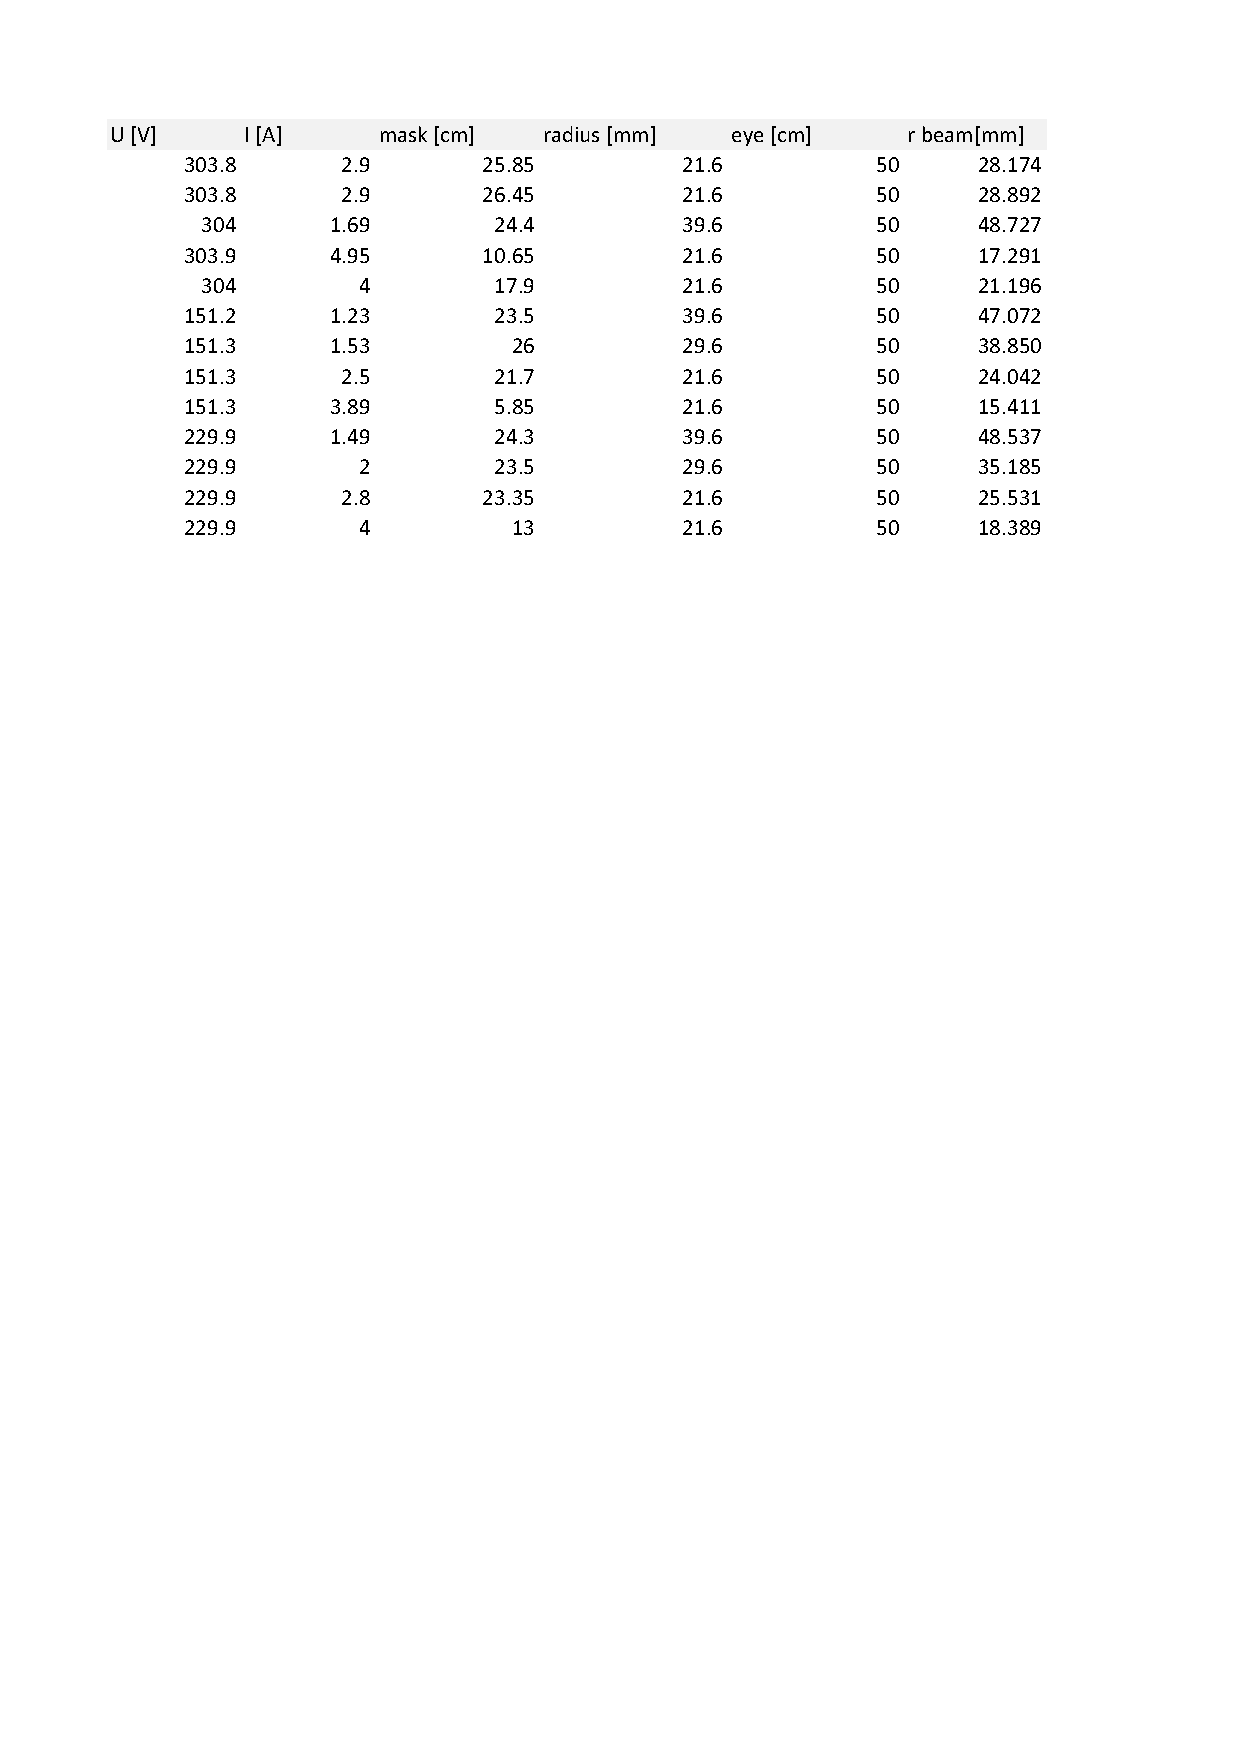
\includegraphics[width=0.9\textwidth]{diag/measurements.pdf}
	\caption{Measured radii $r$ for different values of $U$ and $I$}
	\label{fig:measurements}
\end{figure}

\section{Analysis and Discussion}

\subsection{Sources of error}
\label{sec:error}

\section{Conclusion}

\begin{thebibliography}{9}

\bibitem{physcript13}
  Peter Wurz,
  \emph{Anleitung zum Physikpraktikum}
  FS2013

\end{thebibliography}

\end{document}
